% =====================================================================
%  Synthèse hebdomadaire des tendances médias, solution Power Automate
%  Meriem Sohbi, cas pratique M6, novembre 2026
%  Compilateur Overleaf : pdfLaTeX (par défaut). Trois pages A4,
%  une partie par page. Après chaque modification, vérifier les 3 pages.
% =====================================================================
\documentclass[10pt,a4paper]{article}

% ---------- Mise en page ----------
\usepackage[a4paper,top=13mm,bottom=18mm,left=15mm,right=15mm,footskip=10mm]{geometry}
\usepackage[T1]{fontenc}
\usepackage[utf8]{inputenc}
\usepackage{lmodern}
\IfFileExists{french.ldf}{\usepackage[french]{babel}}{}
\usepackage{microtype}
\usepackage{xcolor}
\usepackage{array,tabularx,booktabs}
\usepackage{enumitem}
\usepackage[most]{tcolorbox}
\usepackage{tikz}
\usetikzlibrary{arrows.meta,positioning,decorations.pathreplacing,calc,babel}
\usepackage{fancyhdr}
\usepackage{lastpage}
\usepackage[hidelinks]{hyperref}

% ---------- Couleurs ----------
\definecolor{teal}{HTML}{1B7A80}
\definecolor{ink}{HTML}{1F2933}
\definecolor{muted}{HTML}{6B7785}
\definecolor{amber}{HTML}{C9821F}
\definecolor{ardoise}{HTML}{2F5D8C}
\definecolor{brique}{HTML}{B04A2F}
\colorlet{tealfond}{teal!8}
\colorlet{tealtrait}{teal!35}
\colorlet{grisfond}{black!4}
\colorlet{gristrait}{black!22}
\colorlet{amberfond}{amber!12}

% ---------- Texte ----------
\setlength{\parindent}{0pt}
\setlength{\parskip}{3pt}
\setlist{nosep,itemsep=1pt}
\setlist[enumerate]{leftmargin=1.4em}

% ---------- Titres ----------
\newcommand{\partie}[2]{%
  {\Large\bfseries #1.\ \textcolor{teal}{#2}}\par\vspace{3pt}
  {\color{black!20}\rule{\linewidth}{0.4pt}}\par\vspace{4pt}}
\newcommand{\lab}[1]{\textbf{#1}}
% Petits titres colorés selon leur sens, toujours suivis de deux-points :
%   \cadre    bleu ardoise : cadrer et planifier (questions, périmètre, pilote)
%   \solution bleu-vert    : ce que fait la solution (déroulement, rôles, données, IA)
%   \humain   ambre        : les personnes (utilisateurs, formation, adoption, transparence)
%   \verif    brique       : ce qui reste incertain ou à vérifier (manques, hypothèses, risques)
% Le bleu-vert et l'ambre ont le même sens que dans les schémas (IA et décision humaine).
\newcommand{\cadre}[1]{\textbf{\color{ardoise}#1 :}}
\newcommand{\solution}[1]{\textbf{\color{teal}#1 :}}
\newcommand{\humain}[1]{\textbf{\color{amber!85!black}#1 :}}
\newcommand{\verif}[1]{\textbf{\color{brique}#1 :}}

% ---------- Encadrés ----------
\newtcolorbox{encadre}{colback=tealfond,colframe=tealtrait,boxrule=0.4pt,arc=3pt,
  left=6pt,right=6pt,top=3pt,bottom=3pt,before skip=4pt,after skip=4pt}
\newtcolorbox{carte}{colback=grisfond,colframe=gristrait,boxrule=0.4pt,arc=3pt,
  left=7pt,right=7pt,top=4pt,bottom=4pt,before skip=3pt,after skip=3pt}

% ---------- Tableaux ----------
\newcolumntype{L}{>{\raggedright\arraybackslash}X}
\renewcommand{\arraystretch}{1.12}

% ---------- Styles des schémas ----------
\tikzset{
  >={Stealth[length=3.2pt]},
  etape/.style={draw=gristrait, fill=grisfond, rounded corners=2pt, line width=0.4pt,
    align=center, inner sep=2.5pt, font=\scriptsize},
  etapeia/.style={etape, draw=teal, fill=tealfond, line width=0.8pt},
  etapehum/.style={etape, draw=amber, fill=amberfond, line width=0.8pt},
  fleche/.style={->, draw=muted, line width=0.45pt}}
\newcommand{\bloc}[2]{\textbf{#1}\\[-0.5pt]{\color{ink!85}#2}}

% ---------- Pied de page ----------
\pagestyle{fancy}
\fancyhf{}
\renewcommand{\headrulewidth}{0pt}
\lfoot{\scriptsize\color{muted}Meriem Sohbi \textperiodcentered{} Cas pratique M6}
\rfoot{\scriptsize\color{muted}\thepage\,/\,\pageref{LastPage}}

\color{ink}
\begin{document}

% =====================================================================
%  EN-TÊTE
% =====================================================================
{\LARGE\bfseries Synthèse hebdomadaire des tendances médias\par}
\vspace{1pt}
{\bfseries Proposition d’une première solution avec Power Automate\par}
\vspace{1pt}
{\small\color{muted}Meriem Sohbi \textperiodcentered{} Cas pratique M6 \textperiodcentered{} Novembre 2026\par}
\vspace{3pt}
{\color{teal}\rule{\linewidth}{1.2pt}}\par\vspace{6pt}

% =====================================================================
%  PAGE 1
% =====================================================================
\partie{1}{Comprendre le besoin et cadrer la première version}

L’équipe de programmation prépare chaque semaine une synthèse à partir de sources publiques et d’informations internes. Elle souhaite gagner du temps sur cette préparation, sans perdre la maîtrise des sources ni du contenu diffusé.

% ---------- Schéma : le travail actuel ----------
\begin{center}
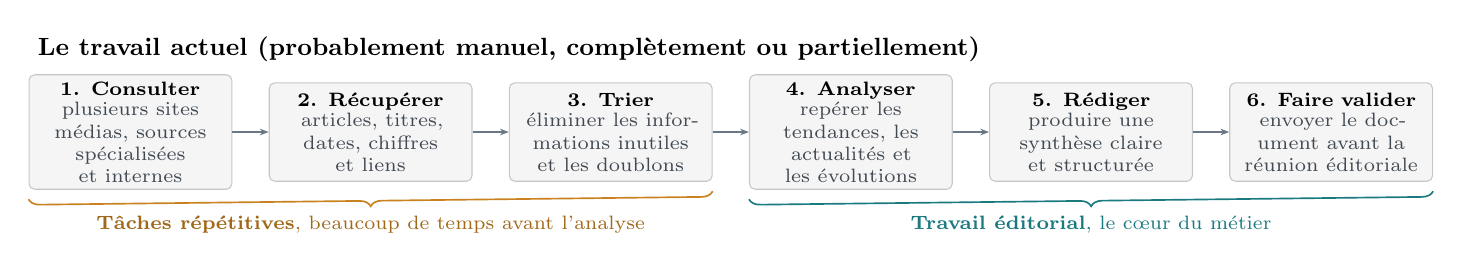
\begin{tikzpicture}[node distance=4.6mm]
  \tikzset{tache/.style={etape, text width=24mm, minimum height=12.5mm}}
  \node[font=\small\bfseries, anchor=west] at (-1.3,1.05) {Le travail actuel (probablement manuel, complètement ou partiellement)};
  \node[tache] (t1) at (0,0) {\bloc{1. Consulter}{plusieurs sites médias, sources spécialisées et internes}};
  \node[tache, right=of t1] (t2) {\bloc{2. Récupérer}{articles, titres, dates, chiffres et liens}};
  \node[tache, right=of t2] (t3) {\bloc{3. Trier}{éliminer les informations inutiles et les doublons}};
  \node[tache, right=of t3] (t4) {\bloc{4. Analyser}{repérer les tendances, les actualités et les évolutions}};
  \node[tache, right=of t4] (t5) {\bloc{5. Rédiger}{produire une synthèse claire et structurée}};
  \node[tache, right=of t5] (t6) {\bloc{6. Faire valider}{envoyer le document avant la réunion éditoriale}};
  \foreach \a/\b in {t1/t2,t2/t3,t3/t4,t4/t5,t5/t6} \draw[fleche] (\a) -- (\b);
  \draw[decorate, decoration={brace, mirror, amplitude=4pt}, draw=amber, line width=0.6pt]
    ($(t1.south west)+(0,-1.2mm)$) -- ($(t3.south east)+(0,-1.2mm)$)
    node[midway, below=4pt, font=\scriptsize, text=amber!80!black] {\textbf{Tâches répétitives}, beaucoup de temps avant l’analyse};
  \draw[decorate, decoration={brace, mirror, amplitude=4pt}, draw=teal, line width=0.6pt]
    ($(t4.south west)+(0,-1.2mm)$) -- ($(t6.south east)+(0,-1.2mm)$)
    node[midway, below=4pt, font=\scriptsize, text=teal] {\textbf{Travail éditorial}, le cœur du métier};
\end{tikzpicture}
\end{center}
\vspace{-8pt}
{\small\color{muted}\verif{Le problème} beaucoup de temps est consacré à des tâches répétitives avant même que le véritable travail éditorial commence.\par}

Je suppose que la collecte et le tri représentent une part importante de ce temps, tandis que le jugement éditorial doit rester humain. L’objectif est donc d’automatiser une partie du travail préparatoire, sans remplacer le rôle du journaliste ou du programmateur, en conservant deux éléments essentiels : la \emph{traçabilité} (savoir exactement d’où vient chaque information) et le \emph{contrôle humain} (aucune synthèse n’est diffusée sans validation).

\begin{encadre}
\solution{En résumé} automatiser la préparation, pas la décision éditoriale.\\
\solution{Résultat attendu} une synthèse hebdomadaire organisée par thèmes, dans laquelle chaque information reste reliée à sa source. Le document est relu, corrigé et validé par un membre de l’équipe avant toute diffusion.
\end{encadre}

\humain{Utilisateurs concernés} la personne chargée de préparer la synthèse la relit et la signe. L’équipe de programmation l’utilise pour préparer ses discussions. Un référent éditorial reste responsable de la sélection finale et de la diffusion.

\cadre{Questions à poser avant de construire}\par\vspace{1pt}
{\small
\begin{tabularx}{\linewidth}{>{\raggedright\arraybackslash}p{0.47\linewidth}L}
\toprule
\textbf{Question} & \textbf{Ce qu’elle permet de préciser}\\
\midrule
Qui utilise la synthèse, quand, et quelles décisions doit-elle éclairer ? & Le format, la longueur, l’heure de livraison et le niveau de détail.\\
Combien d’articles, de sources et de temps sont nécessaires aujourd’hui ? & Le volume à traiter et la situation de départ pour mesurer le gain.\\
Quelles sources sont indispensables, prioritaires et autorisées ? & La liste blanche des sources et les droits à vérifier.\\
Que contient l’API interne, avec quels droits et comment y accéder ? & Les données disponibles, leur format, l’authentification et les contraintes réseau.\\
Quels outils et quelles licences sont déjà disponibles ? & Ce que le flux peut utiliser, donc la faisabilité technique.\\
Quelles informations sont considérées comme pertinentes ? & Des exemples d’articles retenus ou écartés pour définir les critères de tri.\\
\bottomrule
\end{tabularx}}


\verif{Informations manquantes} le format du document partagé, la politique IA de l’entreprise et ses règles de confidentialité, le volume d’articles par semaine, la nature et le nombre des sources, des synthèses déjà réalisées pour servir d’exemples, le temps passé aujourd’hui et les outils disponibles. Les questions ci-dessus permettent d’obtenir ces réponses.

\verif{Hypothèses de travail} Power Automate et Microsoft 365 sont déjà en place, donc je construis dedans (information obtenue lors de l’entretien). Je suppose également que certaines sources publiques proposent un flux RSS et que l’API interne peut être utilisée, avec l’accord de son propriétaire, pour un export interne des audiences. Aucune donnée interne n’est envoyée à l’IA, pour des raisons de confidentialité, et le dernier mot ne revient jamais à l’IA. Ces points restent à confirmer avec les équipes IT et métier.

\cadre{Périmètre de la V1} je commencerais avec quelques sources publiques sélectionnées et une seule source interne, une collecte hebdomadaire, un dédoublonnage simple, la classification et le résumé des contenus, puis la génération d’un brouillon soumis à validation humaine. Les réseaux sociaux, les alertes quotidiennes, la veille en temps réel, l’analyse prédictive et une archive interrogeable seraient étudiés dans un second temps. Cette archive pourrait alors être un bon cas d’usage de RAG.

\solution{Principe de conception} automatiser les tâches répétitives et réserver à l’équipe la décision sur ce qui mérite d’être diffusé.

% =====================================================================
%  PAGE 2
% =====================================================================
\newpage
\partie{2}{Fonctionnement proposé et choix techniques}

Je privilégie un workflow orchestré par Power Automate, à condition que les connecteurs et licences nécessaires soient disponibles dans l’environnement M6. Il enchaîne les étapes sans développer d’application, et un classeur Excel partagé conserve les informations collectées et leur statut. Quand une règle fixe suffit, je n’utilise pas d’IA : la logique tient dans trois Office Scripts.

% ---------- Schéma : fonctionnement proposé ----------
\begin{center}
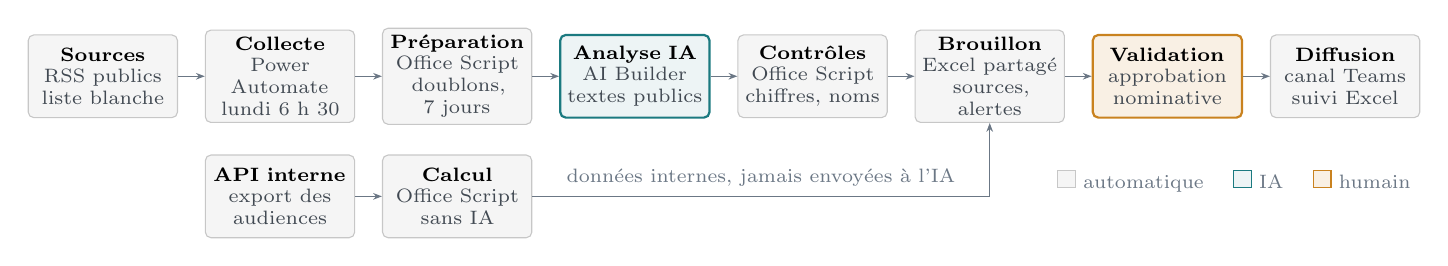
\begin{tikzpicture}[node distance=3.4mm]
  \tikzset{e/.style={etape, text width=17.2mm, minimum height=10.5mm},
           eia/.style={etapeia, text width=17.2mm, minimum height=10.5mm},
           ehum/.style={etapehum, text width=17.2mm, minimum height=10.5mm}}
  \node[e] (s1) at (0,0) {\bloc{Sources}{RSS publics\\liste blanche}};
  \node[e, right=of s1] (s2) {\bloc{Collecte}{Power Automate\\lundi 6~h~30}};
  \node[e, right=of s2] (s3) {\bloc{Préparation}{Office Script\\doublons, 7 jours}};
  \node[eia, right=of s3] (s4) {\bloc{Analyse IA}{AI Builder\\textes publics}};
  \node[e, right=of s4] (s5) {\bloc{Contrôles}{Office Script\\chiffres, noms}};
  \node[e, right=of s5] (s6) {\bloc{Brouillon}{Excel partagé\\sources, alertes}};
  \node[ehum, right=of s6] (s7) {\bloc{Validation}{approbation\\nominative}};
  \node[e, right=of s7] (s8) {\bloc{Diffusion}{canal Teams\\suivi Excel}};
  \foreach \a/\b in {s1/s2,s2/s3,s3/s4,s4/s5,s5/s6,s6/s7,s7/s8} \draw[fleche] (\a) -- (\b);
  \node[e, below=4mm of s2] (i1) {\bloc{API interne}{export des\\audiences}};
  \node[e, right=of i1] (i2) {\bloc{Calcul}{Office Script\\sans IA}};
  \draw[fleche] (i1) -- (i2);
  \draw[fleche] (i2.east) -- (i2.east -| s6.south) -- (s6.south);
  \node[font=\scriptsize, text=muted, above] at ($(i2.east)!0.5!(i2.east -| s6.south)$) {données internes, jamais envoyées à l’IA};
  \node[font=\scriptsize, text=muted, anchor=east] at ($(s8.south east)+(0,-8mm)$)
    {\tikz\fill[grisfond,draw=gristrait] (0,0) rectangle (2.2mm,2.2mm); automatique \quad
     \tikz\fill[tealfond,draw=teal] (0,0) rectangle (2.2mm,2.2mm); IA \quad
     \tikz\fill[amberfond,draw=amber] (0,0) rectangle (2.2mm,2.2mm); humain};
\end{tikzpicture}
\end{center}
\vspace{-6pt}

\solution{Déroulement}
\begin{enumerate}
\item Chaque lundi à 6~h~30, le connecteur RSS récupère, pour chaque source de la liste blanche, les nouveaux titres, dates, liens et, selon les sites, un extrait. Pour les sources sans RSS, une autre méthode autorisée devra être étudiée.
\item Un Office Script garde les sept derniers jours et repère les doublons par l’URL nettoyée ou le titre. Les articles proches sont regroupés sans perdre leurs références, et les chiffres qui diffèrent d’une source à l’autre sont signalés.
\item L’IA propose, pour chaque sujet, une catégorie, un résumé fidèle au texte fourni et les points à vérifier.
\item Un second script contrôle la réponse : chaque chiffre et chaque nom propre doit exister dans la source.
\item Le brouillon est écrit dans le classeur avec les sources, les liens, les contradictions et les alertes. Un responsable le corrige puis l’approuve depuis Teams ou Outlook, et la version validée est publiée dans le canal de l’équipe.
\end{enumerate}

\solution{Répartition des rôles}\par\vspace{1pt}
{\small
\begin{tabularx}{\linewidth}{>{\bfseries}p{0.17\linewidth}L}
\toprule
Automatisation & Déclenchement, collecte, normalisation, détection des doublons, contrôles, calculs, assemblage et notifications.\\
IA & Classification thématique, résumé des textes fournis et signalement des points à vérifier.\\
Humain & Choix des sujets importants, arbitrage des contradictions, vérification du contexte et validation finale.\\
\bottomrule
\end{tabularx}}

\solution{Données} deux circuits séparés. L’IA reçoit uniquement des contenus publics : titre, extrait de 600 caractères au plus, date, source et niveau de fiabilité, sans adresse web. Les données internes, comme les audiences, arrivent par un export dans une table Excel et sont calculées par un script, sans jamais passer par l’IA.

\verif{Prérequis à vérifier} le flux n’utilise que des connecteurs standard (RSS, Excel, Approbations, Teams), à condition que les Office Scripts soient activés et que les règles DLP du tenant les autorisent. L’action IA, un prompt AI Builder, consomme des crédits AI Builder ou Copilot et sa licence reste à confirmer. Pour l’API interne, une connexion directe passe par le connecteur HTTP, qui est premium : je la privilégie si l’API est documentée et autorisée, sinon un export régulier fourni par l’équipe propriétaire sert de solution de repli.

\begin{carte}
\solution{Consigne envoyée à l’IA} « À partir du titre et de l’extrait fournis, propose une catégorie, un résumé de deux phrases maximum et les éléments qui méritent une vérification. Ne crée aucune information qui ne figure pas dans le texte. Si une information manque, indique \emph{non précisé}. Conserve la source et le lien d’origine. »
\end{carte}

\solution{Partie fonctionnelle} je joins les trois Office Scripts, le classeur modèle, le prompt et une fiche de montage du flux en 16 actions. Les scripts passent cinq scénarios de test avec un faux classeur ; le flux lui-même n’a pas pu être monté sans environnement Microsoft 365.

\vspace{2pt}
{\small\bfseries Exemple fictif de synthèse courte}\hfill{\scriptsize\color{muted}Données inventées pour illustrer le résultat}
\begin{carte}
{\large\bfseries Veille médias, semaine du 16 au 22 novembre 2026}\hfill{\footnotesize\bfseries\color{amber}BROUILLON À VALIDER}\par\vspace{2pt}
\solution{À retenir} Chaîne Concurrente 1 annonce une série policière en prime time dès janvier. Plusieurs articles évoquent des formats courts en début de soirée, une tendance à suivre sans conclure à un mouvement généralisé.\par
\solution{Programmation et concurrence} la série comptera six épisodes de 52 minutes, le mardi soir. Question pour la réunion : faut-il contre-programmer ce créneau ?\par
{\scriptsize\color{muted}Sources : communiqué officiel du diffuseur et Flux Médias Pro, liens conservés dans le document.}\par
\solution{Audiences internes, calcul automatique sans IA} Duel de Cuisine \textbf{+14,1~\%} \quad Enquêtes Ouvertes \textbf{$-$22,9~\%}\par
{\scriptsize\color{muted}Source : données internes fictives, évolution par rapport à la semaine précédente.}\par
\verif{À vérifier} la finale du « Grand Défi » aurait réuni 3,1 millions de téléspectateurs selon Flux Médias Pro et 2,8 millions selon Écran Info. Une rumeur sur le non-renouvellement d’une série quotidienne n’est pas confirmée. La source Écran Lab n’a pas pu être collectée, et un article contenant une consigne cachée adressée à l’IA a été écarté.
\end{carte}

% =====================================================================
%  PAGE 3
% =====================================================================
\newpage
\partie{3}{Difficultés, sécurité et droits, risques et mise en place}

\verif{Traitement des principales difficultés}\par\vspace{1pt}
{\small
\begin{tabularx}{\linewidth}{>{\raggedright\arraybackslash}p{0.24\linewidth}L}
\toprule
\textbf{Situation} & \textbf{Réponse prévue}\\
\midrule
Sources contradictoires & Conserver les différentes valeurs, dates et références, et signaler le désaccord. La donnée officielle prime, sinon l’équipe arbitre.\\
Information non vérifiable & Chaque source a un niveau de fiabilité A, B ou C. Une information issue d’une seule source peu fiable porte la mention « à confirmer » et n’est pas présentée comme un fait établi.\\
Doublons & Éliminer les doublons exacts (adresses nettoyées, titres comparés) et regrouper prudemment les articles traitant du même sujet, en conservant chaque source.\\
Source ou API indisponible & Trois tentatives par source, puis journaliser l’échec et afficher une alerte dans Teams. Ne jamais remplacer silencieusement une donnée manquante par une ancienne valeur.\\
Erreur de l’IA & Conserver le texte d’origine et vérifier que chaque chiffre et chaque nom propre existe dans la source. Le résumé peut être corrigé ou rejeté, et une réponse illisible bascule en rédaction manuelle.\\
Consigne cachée dans un texte & Le contenu externe est une donnée non fiable : il ne peut ni modifier les consignes ni déclencher une action. Le texte est écarté et signalé.\\
\bottomrule
\end{tabularx}}

Ces contrôles repèrent un chiffre ou un nom inventé, mais pas un fait mal reformulé avec des mots. C’est pourquoi la relecture humaine reste obligatoire.

\verif{Sécurité et droits à vérifier} avec l’administrateur Power Platform, je vérifierais les droits d’accès à l’API, les règles DLP du tenant pour les connecteurs utilisés, les habilitations SharePoint et la politique interne concernant l’envoi de contenus à un service d’IA. Seuls des extraits publics sont transmis à l’IA dans la V1, et le classeur reste dans l’espace SharePoint de l’équipe. Avec les interlocuteurs juridiques, je vérifierais les conditions d’usage des flux RSS, les droits de réutilisation des articles et les éventuelles licences de revue de presse.

\cadre{Lancement et mesure} je proposerais un pilote de quatre à six semaines avec trois à cinq utilisateurs.
\begin{enumerate}
\item \textbf{Semaine 0 :} mesurer le temps actuel, choisir des exemples de référence et observer de près le fonctionnement actuel. Je testerais aussi la consigne IA à la main sur une semaine passée : si les résumés ne sont pas utiles à la main, ils ne le seront pas automatisés.
\item \textbf{Semaines 1 et 2 :} le brouillon est produit en parallèle de la méthode habituelle, puis comparé et corrigé avec les utilisateurs, en tenant compte des remarques de chacun.
\item \textbf{Semaines 3 à 6 :} l’équipe part du brouillon, et chaque retrait ou correction est noté.
\item \textbf{Fin du pilote :} décision sur des seuils fixés au départ avec l’équipe. Si les résultats sont satisfaisants, l’équipe adopte progressivement le nouveau fonctionnement.
\end{enumerate}

{\small
\begin{tabularx}{\linewidth}{>{\bfseries}p{0.17\linewidth}L}
\toprule
Temps gagné & Temps total de préparation, relecture et correction, avant et pendant le pilote.\\
Qualité & Résumés conservés ou corrigés, erreurs détectées avant diffusion et sujets importants manqués.\\
Utilisation & Nombre d’utilisateurs actifs, fréquence d’utilisation et lecture du brouillon avant la réunion.\\
Coût & Licences, crédits IA consommés et temps de maintenance, comparés au gain obtenu.\\
\bottomrule
\end{tabularx}}

\humain{Faire comprendre l’outil} une ou plusieurs formations, avec une démonstration d’environ 30 minutes, plus longue si nécessaire selon les disponibilités et les besoins de l’équipe, avec des explications simples et des réponses à leurs questions. Elle serait accompagnée d’un document « ce que l’outil fait et ne fait pas ». Chaque élément du brouillon indique pourquoi il a été retenu, avec ses sources et ses alertes, et un référent dans l’équipe recueille les erreurs.

\humain{Si l’outil fonctionne mais reste peu utilisé} je chercherais d’abord la cause avec les utilisateurs, avant de toucher à l’outil : format trop long, manque de pertinence, mauvais moment d’envoi ou manque de confiance. J’adapterais ensuite le format ou le processus avec eux, plutôt que d’ajouter immédiatement de la technologie.

\begin{encadre}
\humain{Transparence} j’ai utilisé des IA génératives (Claude et ChatGPT) pour m’aider à structurer les pistes, clarifier certains choix techniques, écrire les Office Scripts et les tester avec des données fictives, et améliorer une rédaction qui reste la mienne avec mon propre style. Les arbitrages présentés ici sont les miens aussi : rester dans Power Automate avec des connecteurs standard, une V1 limitée, des données traçables, une séparation entre données internes et contenus transmis à l’IA, et une validation humaine obligatoire. Je n’ai pas pu vérifier l’environnement Microsoft 365 de M6, les licences et crédits IA disponibles, l’accès réel à l’API, les autorisations de réutilisation des contenus ni les gains qui seraient obtenus. Le workflow décrit est donc, dans un premier temps, une proposition d’architecture.
\end{encadre}

{\scriptsize\color{muted}\textbf{Références techniques à vérifier lors du cadrage :} documentation Microsoft Learn des connecteurs RSS, Excel Online (Business) et Approbations, des Office Scripts et des licences AI Builder. Les prérequis de licence et de sécurité dépendent de la configuration de l’entreprise.\par}

\end{document}